\documentclass[../../main.tex]{subfiles}
\begin{document}
\section{Implementation}

In the following section, each step of the algorithm  will be described using pseudo code. Then, in order to describe the MapReduce flow, the Pig scripts written for the algorithms are analyzed.


\subsection{Algorithm}
The algorithm takes a few input parameters from the user before running
\begin{itemize}
\item An $N$-sized list of sequences $S={s_0,s_1,\ldots,s_{N-1}}$, each sequence of variable length.
\item $k$-mer size $k$.
\item $H$, the number of hash functions in the sketch
\item $\epsilon$, the threshold for similarity.  
\end{itemize}

Initially, the sequences had to be  transformed into meaningful input for the hash functions used to produce the max-min-wise sketches. Natural numbers fit the purpose well, and are exactly what $k$-mer transformations constitute. The function \texttt{kmerTransformation}($s,k$), as seen in Alg. \ref{alg:trans}, is how the $k$-mer were transformed. \texttt{transformChar} applies the same bit-wise transformation as described in Section \ref{sec:kmertrans}. 

\begin{algorithm}
\caption{Transforms sequence $s$ into its $k$-mer transformation}\label{alg:trans}
\textbf{Input:} a sequence $s$, a $k$-mer size $k$\\
\textbf{Functions:} \texttt{transformChar}($s,k$) maps the character of a $k$-mer to 2-bit values, \texttt{generateKmer}($s,k$) returns all $k$-mers of $s$.\\
\textbf{Output:} The transformed $k$-mer in a list kmerTransformed.
\begin{algorithmic}[1]
\Statex
\Function{kmerTransformation}{$s, k$}
	
	\Let{kmers}{\texttt{generateKmer}($s,k$)} \Comment{saves $k$-mer of $s$}
	\For{kmer \textbf{in} kmers}
		\Let{prod}{1}
		\Let{sum}{0}
		\For{$i \gets 0 \textrm{ to kmer.length } - 1$}
			\Let{sum}{sum + prod $\cdot$ \texttt{transformChar}(gram.charAt(i))}
			\Let{prod}{prod $\cdot$ 4}
		\EndFor
		\State kmersTransformed.append(sum)
	\EndFor
\State \Return{kmersTransformed}
\EndFunction
\end{algorithmic}
\end{algorithm}

Once the transformations were done, a function for producing the max-min-wise sketches for {\bf MM}- and {\bf MM½} was made. As concluded in the Hash Performance Test, the Carter Wegman hash function (Eq. \ref{carterhash}) was most applicable. These hash functions will be referred to as $h_i(x)$ from now on. For the sketch, $H$ hashfunctions are generated for the sketch of {\bf MM} and $H/2$ hash functions for the sketch of {\bf MM½}, each with a different $a$ and $b$. They take the form 
$$
h_i(x)=((a_i\cdot x + b_i) \mod p )\mod 10000
$$
where $a=i+1$, $b=i$, and $p=1845587707$ for $i=0,1,\ldots,H-1$. The $10000$ at the end was to ensure that the change of collision was $0.01\%$, a sufficient precision for the purpose.\\

Alg. \ref{alg:minmax} shows how the max-min-wise sketch for {\bf MM} was produced. It runs through all $H$ hash functions to find the value that is smallest and highest in the transformed $k$-mer list. Alg. \ref{alg:minmaxhalf} shows the pseudocode for calculating max-min-wise sketch for {\bf MM½}, where the only change needed was to divide the number of hash functions by two.

\begin{algorithm}
\caption{Uses transformed $k$-mer to find sketch for {\bf MM} of a sequence}\label{alg:minmax}
\textbf{Input:} a list of transformed $k$-mer $kT$ of a sequence, $H$ number of hashfunctions.\\
\textbf{Parameters:} $h_i(x)$ the ith hash function of the $H$ hash functions initiated.\\
\textbf{Output:} {\bf MM} of a sequence.
\begin{algorithmic}[1]
\Statex
\Function{toMMSketch}{$kT$}
	\Let{MM}{Ø}
	\For{$i \gets 0 \textrm{ to } H - 1$}
		\Let{hmin}{$\infty$}
		\Let{hmax}{$-\infty$}		
		\For{$kt$ in $kT$}
			\Let{val}{$h_i(kt)$}
			\If{val $<$ hmin}
				hmin = val
			\EndIf
			\If{val $>$ hmax}
				hmax = val
			\EndIf
		\EndFor
		\State MM.append([hmin,hmax])
	\EndFor
\State \Return{kmerTransformed}
\EndFunction
\end{algorithmic}
\end{algorithm}

\begin{algorithm}
\caption{Uses transformed $k$-mer to find sketch for {\bf MM½} of a sequence}\label{alg:minmaxhalf}
\textbf{Input:} a list of transformed $k$-mer $kT$ of a sequence, $H$ number of hashfunctions.\\
\textbf{Parameters:} $h_i(x)$ the ith hash function of the $H/2$ hash functions initiated.\\
\textbf{Output:} {\bf MM½} of a sequence.
\begin{algorithmic}[1]
\Statex
\Function{toMMHalfSketch}{$kT$}
	\Let{MMhalf}{Ø}
	\For{$i \gets 0 \textrm{ to } H/2 - 1$}
		\Let{hmin}{$\infty$}
		\Let{hmax}{$-\infty$}		
		\For{$kt$ in $kT$}
			\Let{val}{$h_i(kt)$}
			\If{val $<$ hmin}
				hmin = val
			\EndIf
			\If{val $>$ hmax}
				hmax = val
			\EndIf
		\EndFor
		\State MMhalf.append([hmin,hmax])
	\EndFor
\State \Return{kmerTransformed}
\EndFunction
\end{algorithmic}
\end{algorithm}


As the sketches for {\bf MM} and {\bf MM½} could now be prepared, what remained was to find the Jaccard similarity coefficient of these sketches. Using {\bf MM} and {\bf MM½} as the similarity coefficients, a greedy algorithm was made for each. The greed of the algorithms lies in that if the similarity between two sequences is above $\epsilon$, they are immediately placed in the same cluster, regardless of whether there are other clusters that the other sequence is more similar to. \\

Alg. \ref{alg:minmaxclust} shows the algorithm for {\bf MM} greedy clustering. In line 1-7 the sketches are prepared for the comparison; the remainder is the greedy algorithm. The most interesting part of this algorithm is line 15-22, where the similarity between two strings is determined. Running through all $H$ hash functions, in line 16-20 it checks: if either $h_{min,i}$ or $h_{max,i}$ of both sequences are equal to the other sequence's counterpart, an intersection occurs. When all hash functions have been run through, the similarity between the two strings is determined in line 21 as the intersections over the number of hash functions. If the similarity then surpasses the given $\epsilon$ the strings are placed in the same cluster.\\

Alg. \ref{alg:minmaxhalfclust} has a very similar method as Alg. \ref{alg:minmaxhalfclust}. The main difference lies in line 15-22, where the intersections are determined by the number of $h_{min,i}$ that are equal plus the number of $h_{max,i}$ that are equal. This means that each hash function can result in two intersections, instead of one in Alg. \ref{alg:minmaxclust}. Line 20 finds the similarity, which is the same as in Alg. \ref{alg:minmaxclust}, since the potential number of intersections per hash function is doubled.\\

To render more intelligible the difference between the two algorithms, let us analyze the order of growth of both algorithms.

\subsubsection{Order of Growth: MM}
Each line is analyzed in Alg. \ref{alg:minmaxclust}.\\
line 5: \texttt{kmerTransformation} for a string of length $l$, loops $(l - k + 1)$ times through the string to produce all $k$-mer. Each $k$-mer is then iterated over $k$ times. This takes $\Theta((l-k+1)k)$ time.\\
line 6: \texttt{toMMSketch} for a string of length $l$, repeats $H$ times $(l-k+1)$ comparisons. This takes $\Theta((l-k+1)H)$ time.\\
line 3 - 6: Together, the lines 5 and 6 are repeated $N$ times, giving a runtime of $\Theta(N (l-k+1)(k + H))$.\\
line 8 - 22: Let us first analyse the lower bound. Assuming all sequences will be assigned to the same cluster, line 8 will be run once. Line 12 will be run $N$ times, and line 15 will be run $H$ times per iteration of line 12. The lower bound will therefore be $\Omega(N\cdot H)$. In worst case, all strings belong in different clusters. In this case, line 8 will be run $N$ times, line 12 $N$ times per iteration of line 8, and line 15 $H$ times per iteration of line 12. This gives an upper bound runtime of $O(N^2 \cdot H)$.\\

Conclusively, the runtime will be $\Theta(N (l-k+1)(k + H)) + O(N^2 \cdot H)$. Assuming that $l=1500$\footnote{the limit of length of sequences the program shall be tested on.}, it would necessitate an $N>1500$ to conclusively say that the runtime is $O(N^2 \cdot H)$.
\subsubsection{Order of Growth: MM½}
As the analysis is completely parallel to the one performed for {\bf MM} immediately above, the runtime will be $\Theta(N (l-k+1)(k + H/2)) + O(N^2 \cdot (H/2))$, halving the number of hash functions needed.

\begin{algorithm}
\caption{Greedy Clustering using {\bf MM}}\label{alg:minmaxclust}
\textbf{Input:} a list of DNA/RNA sequences $S=\{s_0,s_1,\ldots,s_{N-1}\}$ of length $N$.\\
\textbf{Parameters:} $H$ number of hash functions, $k$ size of $k$-mer,	$\epsilon$ threshold for string similarity, $c$ current cluster \\
\textbf{Output:} A list of the cluster $C$ each sequence belongs to.
\begin{algorithmic}[1]
\State Initialize $h_i(x)$ for $i=0,1,\ldots,H$
\State Initialize $kT$,$C$, and $MM$ as lists of length $N$
\For{$i \gets 0 \textrm{ to } N -1$}
	\Let{$C$[i]}{0}
	\Let{$kT$[i]}{kmerTransformation($s_i$)}
	\Let{$MM$[i]}{toMMSketch($kT$[i])}
\EndFor
\Let{$c$}{0}
\For{$i \gets 0 \textrm{ to } N - 1$}
	\If{$C$[i] == 0}
		\Let{$c$}{$c$ + 1}
		\Let{$C$[i]}{$c$}
		\For{$j \gets 0 \textrm{ to } N - 1$}
			\Let{$intersections$}{0}
			\If{$C$[i] == 0}
				\For{$k \gets 0 \textrm{ to } H-1$}
					\If{$MM$[i][k][0] == $MM$[j][k][0]}
						\Let{$intersections$}{$intersections + 1$}
					\Else
						\If{$MM$[i][k][1] == $MM$[j][k][1]}
							\Let{$intersections$}{$intersections + 1$}
						\EndIf
					\EndIf
				\EndFor
				\If{$\frac{intersections}{H} \geq \epsilon$}
					\Let{$C$[j]}{$C$[i]}				
				\EndIf
			\EndIf
		\EndFor
	\EndIf
\EndFor
\end{algorithmic}
\end{algorithm}

\begin{algorithm}
\caption{Greedy Clustering using {\bf MM½}}\label{alg:minmaxhalfclust}
\textbf{Input:} a list of DNA/RNA sequences $S=\{s_0,s_1,\ldots,s_{N-1}\}$ of length $N$.\\
\textbf{Parameters:} $H$ number of hash functions, $k$ size of $k$-mer,	$\epsilon$ threshold for string similarity, $c$ current cluster \\
\textbf{Output:} A list of the cluster $C$ each sequence belongs to.
\begin{algorithmic}[1]
\State Initialize $h_i(x)$ for $i=0,1,\ldots,H/2$
\State Initialize $kT$,$C$, and $MM$ as lists of length $N$
\For{$i \gets 0 \textrm{ to } N -1$}
	\Let{$C$[i]}{0}
	\Let{$kT$[i]}{kmerTransformation($s_i$)}
	\Let{$MM$[i]}{toMMhalfSketch($kT$[i])}
\EndFor
\Let{$c$}{0}
\For{$i \gets 0 \textrm{ to } N - 1$}
	\If{$C$[i] == 0}
		\Let{$c$}{$c$ + 1}
		\Let{$C$[i]}{$c$}
		\For{$j \gets 0 \textrm{ to } N - 1$}
			\Let{$intersections$}{0}
			\If{$C$[i] == 0}
				\For{$k \gets 0 \textrm{ to } H/2-1$}
					\If{$MM$[i][k][0] == $MM$[j][k][0]}
						\Let{$intersections$}{$intersections + 1$}
					\EndIf
					\If{$MM$[i][k][1] == $MM$[j][k][1]}
						\Let{$intersections$}{$intersections + 1$}
					\EndIf
				\EndFor
				\If{$\frac{intersections}{H} \geq \epsilon$}
					\Let{$C$[j]}{$C$[i]}				
				\EndIf
			\EndIf
		\EndFor
	\EndIf
\EndFor
\end{algorithmic}
\end{algorithm}
\newpage

\subsection{MapReduce Framework}
In order to parallellize and distribute the algorithm, MapReduce was used. Fig. \ref{fig:mapredflow} shows the flow of this setup. The fasta file is first partitioned, so that each sequence is assigned to a worker. Then, each sequence has the transformation from sequence to sketch performed in parallel. When this transformation is done, all the sequences are passed to the Greedy Clustering algorithm at once, where the clusters are found. Finally, this is saved into an output.

\begin{figure}[h]
\centering
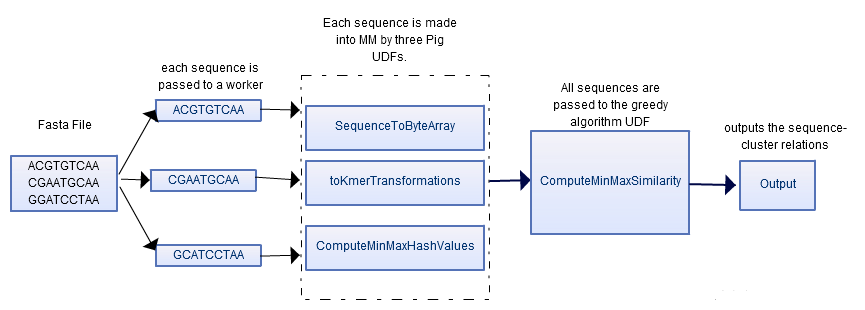
\includegraphics[scale=0.5]{data/MapReduce}
\caption{The flow of the MapReduce FrameWork}\label{fig:mapredflow}
\end{figure}

For the development of the MapReduce framework, Pig Latin was used. Pig Latin is a high level language for compiling and executing MapReduce jobs over Hadoop, in which Pig scripts can be written. Advantageous when performing a pipeline of MapReduce jobs~\cite{pig}, it also demands very few lines of code compared to Hadoop MapReduce code. Additionally, users may write User Defined Functions (abbr. UDF), completely eliminating the need to write any map or reduce function, as they are on the lower level.\\

The Pig script used to create this flow for the {\bf MM} algorithm can be seen in Alg. \ref{alg:pigscript}. All functions that are not uppercase in the Pig script are all user defined functions (UDFs) that were developed in the course of this paper. A closer examination of these UDFs will follow for comprehension of the work load behind it.\\

Before getting into the UDF, we should examine the datatypes of Pig Latin. The only variables that are allowed in a script are DataBags. These are unordered lists of data which contain all data gotten from an operation. As they are spillable, they register with a memory manager which allows for data of greater size than the available memory in a DataBag. These DataBags can then be parsed to a few SQL-like functions such as FILTER, FOREACH, LOAD or GROUP.\\

A noteworthy feature of these four functions is that they only run on a single element of the DataBag. For instance, LOAD first partitions the \$INPUT file by newlines, and then parses it to the function right to USING. The same is the case for FOREACH, which takes each element of a databag and GENERATES and output using an inherent Pig function or UDF to the right of GENERATE. The resulting output of each element is then gathered into a single DataBag, e.g. sequences in Alg. \ref{alg:pigscript}. Within the UDF an additional datatype is allowed, which are Tuples. These are ordered lists of data, or virtually the array of Pig Latin. Tuples only exist within Pig UDFs, and are considered DataBags once they exit the UDF and go into the Pig Latin domain.  
\begin{algorithm}
\caption{Pig script for MapReduce {\bf MM} Greedy Cluster Algorithm}\label{alg:pigscript}
\textbf{Input:} a list of DNA/RNA sequences $S=\{s_0,s_1,\ldots,s_{N-1}\}$ of length $N$.\\
\textbf{Parameters:} \$HASH\_SIZE number of hash functions, \$KMER\_SIZE size of $k$-mer,	\$THRESHOLD is $\epsilon$\\
\textbf{Output:} list of the cluster each sequence belongs to in \textbf{results}.
\begin{algorithmic}[1]
\State sequences = LOAD '\$INPUT' USING FastaReader AS (line: chararray);
\State converted = FOREACH sequences GENERATE SequenceToByteArray(line, \$PROGRAM);
\State NoN = FILTER converted BY byteSeq is not null;
\State kmers = FOREACH NoN GENERATE toKmerTransformations(byteSeq, \$KMER\_SIZE);
\State minmaxvalues = FOREACH kmers GENERATE FLATTEN (ComputeMaxMinHashValues (kmerlist, \$HASH\_SIZE, \$KMER\_SIZE));
\State grouped = GROUP minmaxvalues ALL;
\State a\_count = FOREACH grouped GENERATE COUNT (minmaxvalues);
\State results = FOREACH grouped GENERATE FLATTEN (ComputeMaxMinSimilarity (minmaxvalues, a\_count.\$0, \$HASH\_SIZE, \$THRESHOLD));
\State STORE results into \$OUTPUT;
\end{algorithmic}
\end{algorithm}
\subsection{Pig Script Analysis}

Pig scripts allow three languages to develop UDFs in: Python, Java, and javascript. Of these three, Java was chosen as it was the language with most features available for developing Pig UDFs. We shall examine each line to understand the purpose and thoughts behind each UDF.\\

In line 1, we are loading input from an \$INPUT file using FastaReader. FastaReader was the only function not developed by the author, and is an open source input reader function\footnote{\url{http://cs.gmu.edu/~mlbio/MrMC-MinH/}} which can read fasta files so that each sequence is read as a single line. This means that if sequences span multiple lines, they are gathered by the FastaReader into a single line.\\

SequenceToByteArray then converts each sequence into a byte array using the same bitwise transformation as in the Additional Tools section, describing $k$-mer transformation. If the character N shows up, the sequence is returned as null since none of the test data that were used in this paper had any N present. The lines that hold an unknown character N are then filtered away in line 3.\\

In line 4 the $k$-mer for each sequence are made. The UDF toKmerTransformation was developed so that the output would be the same as using Alg. \ref{alg:trans}. This transformation was used as it was the optimal way of obtaining $k$-mers so that they took as little space as possible. In addition, using this implementation over \texttt{substring} is slightly quicker, as finding the transformed $k$-mer only requires a few multiplications in lieu of splitting strings.\\ 

For transforming the $k$-mers into {\bf MM} sketches, the UDF ComputeMaxMinSimilarity was developed. It follows the exact same formula as Alg. \ref{alg:minmax}, so that a Tuple is filled, in order, with a tuple of two elements containing the maximal and minimal hashed value of each hash function. The maximal and minimal hash value are both integers, as the hash functions are modulused with 10000 in the end, meaning that it would be pointless to use longs.\\

In line 6 and 7 two purposes are serves. Line 6 allowed to make a databag which in only one layer contained all tuples calculated in line 5. With this trick, it was rendered possible to let the FOREACH in line 8 only run once, as the \texttt{grouped} variable contains a DataBag with a single Tuple of all max- and minhashes of all sequences. Line 7 then uses line 6 to calculate the number of seuqences that have been transformed. By finding the number of sequences using line 7, and not simply calculating it in the UDF in line 8, it became possible to use MapReduce to find the number of sequences. This was faster than doing it in a single threaded UDF.\\

Finally, line 8 only runs once to fill the \texttt{results} variable. As the FOREACH only runs once, the advantage of MapReduce is eliminated, since only one worker is allowed to run ComputeMaxMinSimilarity. Unfortunately, there was no way of making it possible to compare each sequence to all other sequences in a MapReduce framework using Pig, since FOREACH cannot parse the entirety of a DataBag several times. Therefore, ComputeMaxMinSimilarity is only run once, and it runs the greedy algorithm as described in Alg. \ref{alg:minmaxclust} line 7-22. It then returns a Tuple containing information on the cluster each sequence is located in. A notable difficulty that came into the creation of this algorithm was that in the beginning, the {\bf MM½} algorithm ran much slower than the {\bf MM}. After rigorous debugging, a hidden side effect of either the way Pig Latin handles Java UDF or JAVA itself turned out to cause this difference in speed.

In line 9, this Tuple is then stored into an \$OUTPUT file.

The development of the {\bf MM½} Pig script was almost identical to that of {\bf MM}. The only differences is that the UDF used in line 8 was ComputeMaxMinHalfSimilarity instead. It follows the greedy algorithm described in \ref{alg:minmaxhalfclust} line 8-21. In the initial stages of development, i had written the Java version so that line 16-19 in Alg. \ref{alg:minmaxhalfclust} was written as

\begin{lstlisting}
if(minhashArray[i][k] == minhashArray[j][k]){
	intersections++;
}
if(maxhashArray[i][k] == maxhashArray[j][k]){
	intersections++;
}
\end{lstlisting}

The corresponding line in ComputeMinMaxSimilarity for {\bf MM} was

\begin{lstlisting}
intersections = (minhashArray[i][k] == minhashArray[j][k] || maxhashArray[i][k] == maxhashArray[j][k]) ? intersections + 1 : intersections;
\end{lstlisting}

Repeadedly, the runs of {\bf MM½} were slower than those of {\bf MM} for the same input, $k$ and $H$, which theoretically made no sense. After a rigorous debugging, changing the above two if statements into the following two lines

\begin{lstlisting}
intersections = (minhashArray[i][k] == minhashArray[j][k]) ? intersections + 1 : intersections;
intersections = (maxhashArray[i][k] == maxhashArray[j][k]) ? intersections + 1 : intersections;
\end{lstlisting}

increased the speed of {\bf MM½} to realistically approximately double the speed of {\bf MM}. This change in the implementation could not have been predicted to have such an influence on the runtime of the Pig scripts. The above was a perfect example of a hidden side effect of the language, for we see that the explicit if statements semantically are identical to the two '?' if statements, but still the '?' have a much faster runtime. While I may not have been able to determine all the hidden side effects in the implementation, as many were tried to be determined as possible.\\

Now that the considerations behind the algorithms, and their implementation have been describe, the testing of the implementation may begin.
\end{document}